\documentclass{standalone}

\usepackage{tikz}
\usepackage{../../style/csmacros}

\definecolor{EDFLBlue}{RGB}{0,112,192}
\definecolor{EDFDBlue}{RGB}{9,53,122}
\definecolor{EDFDOrange}{RGB}{254,88,21}
\definecolor{EDFLOrange}{RGB}{243,157,0}
\definecolor{EDFGreen}{RGB}{80,158,47}
\definecolor{EDFGrey}{RGB}{127,127,127}

\begin{document}
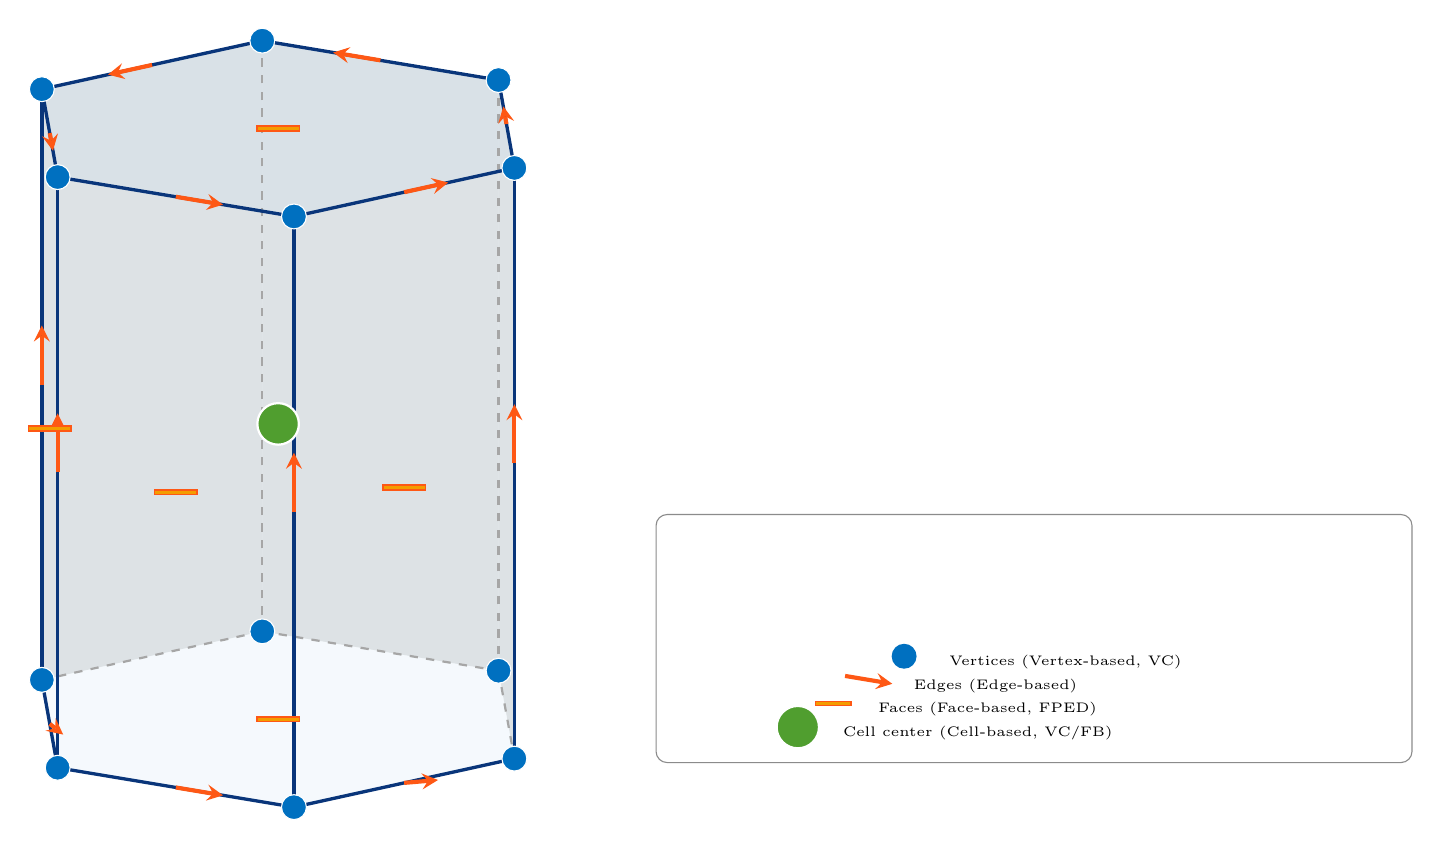
\begin{tikzpicture}[x={(1.2cm, -0.2cm)}, y={(0.6cm, 0.4cm)}, z={(0cm, 1.5cm)}, scale=2.5, >=stealth]

  % Coordinates of the base vertices (z=0)
  \coordinate (B0) at (1.0, 0.0, 0.0);
  \coordinate (B1) at (0.5, 0.866, 0.0);
  \coordinate (B2) at (-0.5, 0.866, 0.0);
  \coordinate (B3) at (-1.0, 0.0, 0.0);
  \coordinate (B4) at (-0.5, -0.866, 0.0);
  \coordinate (B5) at (0.5, -0.866, 0.0);

  % Coordinates of the top vertices (z=2)
  \coordinate (T0) at (1.0, 0.0, 2.0);
  \coordinate (T1) at (0.5, 0.866, 2.0);
  \coordinate (T2) at (-0.5, 0.866, 2.0);
  \coordinate (T3) at (-1.0, 0.0, 2.0);
  \coordinate (T4) at (-0.5, -0.866, 2.0);
  \coordinate (T5) at (0.5, -0.866, 2.0);

  % Midpoints of base edges (z=0)
  \coordinate (MB01) at (0.75, 0.433, 0.0);
  \coordinate (MB12) at (0.0, 0.866, 0.0);
  \coordinate (MB23) at (-0.75, 0.433, 0.0);
  \coordinate (MB34) at (-0.75, -0.433, 0.0);
  \coordinate (MB45) at (0.0, -0.866, 0.0);
  \coordinate (MB50) at (0.75, -0.433, 0.0);

  % Midpoints of top edges (z=2)
  \coordinate (MT01) at (0.75, 0.433, 2.0);
  \coordinate (MT12) at (0.0, 0.866, 2.0);
  \coordinate (MT23) at (-0.75, 0.433, 2.0);
  \coordinate (MT34) at (-0.75, -0.433, 2.0);
  \coordinate (MT45) at (0.0, -0.866, 2.0);
  \coordinate (MT50) at (0.75, -0.433, 2.0);

  % Midpoints of vertical edges (z=1)
  \coordinate (MV0) at (1.0, 0.0, 1.0);
  \coordinate (MV1) at (0.5, 0.866, 1.0);
  \coordinate (MV2) at (-0.5, 0.866, 1.0);
  \coordinate (MV3) at (-1.0, 0.0, 1.0);
  \coordinate (MV4) at (-0.5, -0.866, 1.0);
  \coordinate (MV5) at (0.5, -0.866, 1.0);

  % Centers of faces
  \coordinate (FC_Bottom) at (0.0, 0.0, 0.0);
  \coordinate (FC_Top) at (0.0, 0.0, 2.0);
  \coordinate (FC_01) at (0.75, 0.433, 1.0);
  \coordinate (FC_12) at (0.0, 0.866, 1.0);
  \coordinate (FC_23) at (-0.75, 0.433, 1.0);
  \coordinate (FC_34) at (-0.75, -0.433, 1.0);
  \coordinate (FC_45) at (0.0, -0.866, 1.0);
  \coordinate (FC_50) at (0.75, -0.433, 1.0);

  % Cell Center
  \coordinate (CC) at (0.0, 0.0, 1.0);

  % Draw Back Faces / Shading
  \fill[EDFGrey, opacity=0.3] (B3) -- (B2) -- (T2) -- (T3) -- cycle;
  \fill[EDFGrey, opacity=0.3] (B2) -- (B1) -- (T1) -- (T2) -- cycle;
  \fill[EDFGrey, opacity=0.3] (B1) -- (B0) -- (T0) -- (T1) -- cycle;

  % Draw Front Faces / Shading for better 3D depth
  \fill[EDFLBlue!10, opacity=0.4] (B3) -- (B4) -- (T4) -- (T3) -- cycle;
  \fill[EDFLBlue!10, opacity=0.4] (B4) -- (B5) -- (T5) -- (T4) -- cycle;
  \fill[EDFLBlue!10, opacity=0.4] (B5) -- (B0) -- (T0) -- (T5) -- cycle;
  \fill[EDFLBlue!15, opacity=0.5] (T0) -- (T1) -- (T2) -- (T3) -- (T4) -- (T5) -- cycle;

  % Draw Hidden (Dashed) Primal Edges
  \draw[gray!70, dashed, line width=0.8pt] (B3) -- (B2);
  \draw[gray!70, dashed, line width=0.8pt] (B2) -- (B1);
  \draw[gray!70, dashed, line width=0.8pt] (B1) -- (B0);
  \draw[gray!70, dashed, line width=0.8pt] (B2) -- (T2);
  \draw[gray!70, dashed, line width=0.8pt] (B1) -- (T1);

  % Draw Visible (Solid) Primal Edges
  \draw[EDFDBlue, line width=1.2pt] (B3) -- (B4);
  \draw[EDFDBlue, line width=1.2pt] (B4) -- (B5);
  \draw[EDFDBlue, line width=1.2pt] (B5) -- (B0);
  \draw[EDFDBlue, line width=1.2pt] (B3) -- (T3);
  \draw[EDFDBlue, line width=1.2pt] (B4) -- (T4);
  \draw[EDFDBlue, line width=1.2pt] (B5) -- (T5);
  \draw[EDFDBlue, line width=1.2pt] (B0) -- (T0);

  % Draw Top Hexagon Base (all solid/visible)
  \draw[EDFDBlue, line width=1.2pt] (T0) -- (T1) -- (T2) -- (T3) -- (T4) -- (T5) -- cycle;

  % --- DEGREES OF FREEDOM ---

  % 1. Vertex-based DoFs (VPCD / VC) - represented by BLUE dots
  \foreach \v in {B0, B1, B2, B3, B4, B5, T0, T1, T2, T3, T4, T5} {
    \fill[EDFLBlue] (\v) circle (1.8pt);
    \draw[white, line width=0.4pt] (\v) circle (1.8pt);
  }

  % 2. Edge-based DoFs (EPFD) - represented by RED/ORANGE arrows along the edges
  % We draw small arrows centered at the midpoint of each edge
  \draw[EDFDOrange, -stealth, line width=1.5pt] (MB34) -- ++(0.1, -0.0866, 0.0);
  \draw[EDFDOrange, -stealth, line width=1.5pt] (MB45) -- ++(0.2, 0.0, 0.0);
  \draw[EDFDOrange, -stealth, line width=1.5pt] (MB50) -- ++(0.1, 0.0866, 0.0);

  \draw[EDFDOrange, -stealth, line width=1.5pt] (MT01) -- ++(-0.1, 0.173, 0.0);
  \draw[EDFDOrange, -stealth, line width=1.5pt] (MT12) -- ++(-0.2, 0.0, 0.0);
  \draw[EDFDOrange, -stealth, line width=1.5pt] (MT23) -- ++(-0.1, -0.173, 0.0);
  \draw[EDFDOrange, -stealth, line width=1.5pt] (MT34) -- ++(0.1, -0.173, 0.0);
  \draw[EDFDOrange, -stealth, line width=1.5pt] (MT45) -- ++(0.2, 0.0, 0.0);
  \draw[EDFDOrange, -stealth, line width=1.5pt] (MT50) -- ++(0.1, 0.173, 0.0);

  \draw[EDFDOrange, -stealth, line width=1.5pt] (MV0) -- ++(0.0, 0.0, 0.2);
  \draw[EDFDOrange, -stealth, line width=1.5pt] (MV3) -- ++(0.0, 0.0, 0.2);
  \draw[EDFDOrange, -stealth, line width=1.5pt] (MV4) -- ++(0.0, 0.0, 0.2);
  \draw[EDFDOrange, -stealth, line width=1.5pt] (MV5) -- ++(0.0, 0.0, 0.2);

  % 3. Face-based DoFs (FPED) - represented by ORANGE squares/diamonds at the center of each face
  \foreach \f in {FC_Top, FC_Bottom, FC_34, FC_45, FC_50} {
    \fill[EDFLOrange] (\f) +(-0.06,-0.06) rectangle +(0.06,0.06);
    \draw[EDFDOrange, line width=0.6pt] (\f) +(-0.06,-0.06) rectangle +(0.06,0.06);
  }

  % 4. Cell-based DoF - represented by a GREEN circle inside the cell center
  \fill[EDFGreen] (CC) circle (3pt);
  \draw[white, line width=0.8pt] (CC) circle (3pt);
  \node[above right] at (CC) {\footnotesize $\celli$};

  % Legend or Labels
  \begin{scope}[shift={(1.8, 1.2, 0.0)}]
    \fill[white, draw=EDFGrey, opacity=0.9, rounded corners] (-0.3, -1.0) rectangle (1.0, 2.8);

    % Vertices
    \fill[EDFLBlue] (0.0, 0.5) circle (1.8pt);
    \node[right] at (0.15, 0.5) {\tiny Vertices (Vertex-based, VC)};

    % Edges
    \draw[EDFDOrange, -stealth, line width=1.5pt] (-0.1, 0.2) -- (0.1, 0.2);
    \node[right] at (0.15, 0.2) {\tiny Edges (Edge-based)};

    % Faces
    \fill[EDFLOrange] (0.0, -0.1) +(-0.05,-0.05) rectangle +(0.05,0.05);
    \draw[EDFDOrange, line width=0.5pt] (0.0, -0.1) +(-0.05,-0.05) rectangle +(0.05,0.05);
    \node[right] at (0.15, -0.1) {\tiny Faces (Face-based, FPED)};

    % Cell
    \fill[EDFGreen] (0.0, -0.4) circle (3.0pt);
    \draw[white, line width=0.5pt] (0.0, -0.4) circle (3.0pt);
    \node[right] at (0.15, -0.4) {\tiny Cell center (Cell-based, VC/FB)};
  \end{scope}

\end{tikzpicture}
\end{document}
